\documentclass[aspectratio=169]{beamer}
\usetheme{Madrid}

% Lato is used on Overleaf; fall back to Helvetica if it is not installed locally.
\IfFileExists{lato.sty}{\usepackage[default]{lato}}{\usepackage{helvet}\renewcommand{\familydefault}{\sfdefault}}
\usepackage{booktabs}
\usepackage{array}
\newcolumntype{L}[1]{>{\raggedright\arraybackslash}p{#1}}
\usepackage{graphicx}
\usepackage{xcolor}
\usepackage{tikz}
\usetikzlibrary{shapes.geometric, arrows.meta, positioning}
\usepackage{amsmath}
\usepackage[T1]{fontenc}
\usepackage[utf8]{inputenc}
\usepackage[english]{babel}

% Real spaces and Unicode text in the PDF, so copy-paste and search work.
\input{glyphtounicode}
\pdfgentounicode=1
\pdfinterwordspaceon

\graphicspath{{../figures/}}

% ── Colours ──────────────────────────────────────────────────────────────────
\definecolor{nlpblue}{HTML}{032A54}
\definecolor{nlplightblue}{HTML}{D6E4F0}
\definecolor{nlpbluemid}{HTML}{0A4A8A}

% ── Override Madrid → nlpblue ─────────────────────────────────────────────────
\setbeamercolor{palette primary}{bg=nlpblue, fg=white}
\setbeamercolor{palette secondary}{bg=nlpblue!85!black, fg=white}
\setbeamercolor{palette tertiary}{bg=nlpblue!70!black, fg=white}
\setbeamercolor{palette quaternary}{bg=nlpblue, fg=white}
\setbeamercolor{structure}{fg=nlpblue}
\setbeamercolor{section in toc}{fg=nlpblue}
\setbeamercolor{block title}{bg=nlpblue, fg=white}
\setbeamercolor{block body}{bg=nlplightblue, fg=black}
\setbeamercolor{itemize item}{fg=nlpblue}
\setbeamercolor{itemize subitem}{fg=nlpblue!70}

% ── Presentation metadata ────────────────────────────────────────────────────
\title[Predicting IMO Performance]{%
  Predicting IMO Performance from\\
  Prior International Olympiad Results}
\author[A.-M.-I. Bogdan]{Ana-Maria-Iulia Bogdan}
\institute[NUSTPB · ACS]{Faculty of Automatic Control and Computers\\
  National University of Science and Technology POLITEHNICA Bucharest}
\date[IAPD · Phase 1]{IAPD Project · Phase 1}

\setbeamertemplate{navigation symbols}{}

\begin{document}

% ── SLIDE 0: Title ────────────────────────────────────────────────────────────
{
\setbeamertemplate{headline}{}
\begin{frame}
  \begin{tikzpicture}[remember picture, overlay]
    \node[anchor=north, yshift=-6pt, text=nlpblue, align=center,
          font=\footnotesize, text width=0.78\paperwidth]
      at (current page.north)
      {National University of Science and Technology POLITEHNICA Bucharest\\
       Faculty of Automatic Control and Computers};
    \node[anchor=north east, xshift=-6pt, yshift=-6pt] at (current page.north east)
      {
\includegraphics[height=1.4cm]{nlp_group_logo.png}};
  \end{tikzpicture}

  \vspace{1.2cm}
  \begin{center}
    {\color{nlpblue}\Large\bfseries
      Predicting IMO Performance from\\[6pt]
      Prior International Olympiad Results}

    \vspace{0.3cm}
    {\color{nlpblue}\normalsize Phase 1: dataset, descriptive statistics and baselines}

    \vspace{0.5cm}
    {\color{nlpblue!30}\rule{0.6\textwidth}{0.4pt}}

    \vspace{0.5cm}
    {\normalsize\textbf{Ana-Maria-Iulia Bogdan}}\\[6pt]
    {\footnotesize\color{nlpblue} MSc Data Science, Faculty of Automatic Control and Computers\\
      National University of Science and Technology POLITEHNICA Bucharest}\\[10pt]
    {\footnotesize\color{gray} IAPD · November 2026}
  \end{center}
\end{frame}
}

% ── SLIDE 1: Motivation ───────────────────────────────────────────────────────
\begin{frame}{Motivation and Research Questions}
  \begin{columns}[T]
    \column{0.52\textwidth}
      \footnotesize
      \begin{itemize}\setlength{\itemsep}{8pt}
        \item The \textbf{IMO}: $\sim$600 pre-university contestants a year,
              6 proof problems $\times$ 7 points, about half receive medals
        \item Results are used as a \textbf{measuring instrument}: to select
              national teams and, recently, to benchmark LLM reasoning
        \item Both uses assume a result reflects a \textbf{stable ability},
              not one noisy exam
        \item Most contestants compete \textbf{before} the IMO: JBMO, BMO, EGMO,
              RMM, APMO, MEMO, PAMO
        \item \textbf{Gap}: prior work is descriptive (Berg, 2021), country-level,
              or predicts careers \emph{from} the IMO (Agarwal \& Gaulé, 2020);
              no study predicts individual IMO results from other olympiads
      \end{itemize}

    \column{0.45\textwidth}
      \begin{block}{Research questions}
        \footnotesize
        \begin{itemize}\setlength{\itemsep}{6pt}
          \item[\textbf{RQ1}] How accurately can a contestant's IMO \textbf{score
                and medal} be predicted from their prior international results
                and their country's history?
          \item[\textbf{RQ2}] Which prior competitions carry the most
                \textbf{predictive signal}?
          \item[\textbf{RQ3}] For whom do predictions \textbf{fail}, and are the
                errors systematic?
        \end{itemize}
      \end{block}
      \vspace{4pt}
      \footnotesize Using \textbf{only information available before} each IMO.
  \end{columns}
\end{frame}

% ── SLIDE 2: Sources and crawling ─────────────────────────────────────────────
\begin{frame}{Data Acquisition: Sources and Crawling}
  \footnotesize
  \setlength{\tabcolsep}{4pt}
  \begin{tabular}{L{2.8cm}L{4.8cm}L{5.4cm}c}
    \toprule
    \textbf{Source} & \textbf{Content} & \textbf{How it is collected} & \textbf{Requests} \\
    \midrule
    \texttt{imo-official.org} & IMO 2000--2026: problem scores, rank, award,
      official contestant id
      & one page per year; JSON embedded in the HTML & 27 \\[2pt]
    \texttt{moresults.org} & 9 olympiads, 1959--2026; profiles linking a
      person's participations
      & client-side app: data file found in its JS bundle, downloaded once
        (not 21,590 pages) & 4 \\[2pt]
    JBMO organisers & JBMO 2018--2020, 2022 (missing above); 2020 with every
      contestant
      & PDFs + HTML; codes (\texttt{ROM2}) mapped to the team pages & 40 \\
    \bottomrule
  \end{tabular}

  \vspace{6pt}
  \begin{columns}[T]
    \column{0.48\textwidth}
      \begin{block}{Crawling etiquette}
        \footnotesize
        \begin{itemize}\setlength{\itemsep}{2pt}
          \item \texttt{robots.txt} checked: both sites allow crawling
          \item Descriptive user agent, 3 s between requests
          \item Local cache: no page is requested twice
        \end{itemize}
      \end{block}
    \column{0.48\textwidth}
      \begin{block}{Privacy}
        \footnotesize
        \begin{itemize}\setlength{\itemsep}{2pt}
          \item Names used only for linking, inside a local cache
          \item Published tables: salted-hash ids, no names
          \item Source PDFs kept locally, cited, not committed
        \end{itemize}
      \end{block}
  \end{columns}
\end{frame}

% ── SLIDE 3: Record linkage ───────────────────────────────────────────────────
\begin{frame}{Building the Dataset: Record Linkage}
  \begin{columns}[T]
    \column{0.52\textwidth}
      \vspace{4pt}
      \scalebox{0.86}{%
      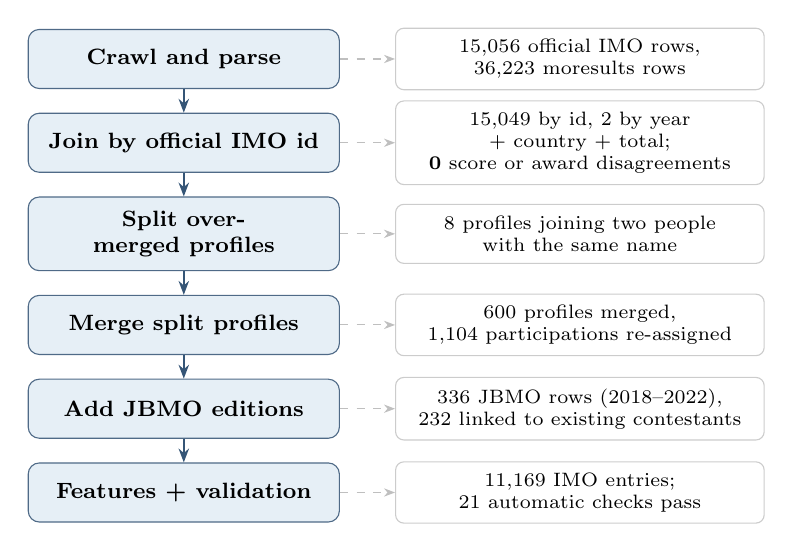
\begin{tikzpicture}[
        node distance=0.30cm and 0.7cm,
        main/.style={rectangle, rounded corners=4pt, draw=nlpblue!70,
                     fill=nlplightblue!60, text width=3.6cm, align=center,
                     font=\footnotesize\bfseries, minimum height=0.75cm, inner sep=5pt},
        data/.style={rectangle, rounded corners=3pt, draw=gray!40,
                     fill=white, text width=4.4cm, align=center,
                     font=\scriptsize, minimum height=0.75cm, inner sep=4pt},
        arr/.style={-{Stealth[length=5pt]}, thick, nlpblue!80},
        darr/.style={-{Stealth[length=4pt]}, dashed, gray!50},
      ]
      \node[main] (s1) {Crawl and parse};
      \node[main, below=of s1] (s2) {Join by official IMO id};
      \node[main, below=of s2] (s3) {Split over-merged profiles};
      \node[main, below=of s3] (s4) {Merge split profiles};
      \node[main, below=of s4] (s5) {Add JBMO editions};
      \node[main, below=of s5] (s6) {Features + validation};
      \node[data, right=of s1] (d1) {15,056 official IMO rows,\\ 36,223 moresults rows};
      \node[data, right=of s2] (d2) {15,049 by id, 2 by year + country + total;\\
                                     \textbf{0} score or award disagreements};
      \node[data, right=of s3] (d3) {8 profiles joining two people\\ with the same name};
      \node[data, right=of s4] (d4) {600 profiles merged,\\ 1,104 participations re-assigned};
      \node[data, right=of s5] (d5) {336 JBMO rows (2018--2022),\\ 232 linked to existing contestants};
      \node[data, right=of s6] (d6) {11,169 IMO entries;\\ 21 automatic checks pass};
      \foreach \a/\b in {s1/s2, s2/s3, s3/s4, s4/s5, s5/s6} \draw[arr] (\a) -- (\b);
      \foreach \i in {1,...,6} \draw[darr] (s\i.east) -- (d\i.west);
      \end{tikzpicture}}

    \column{0.46\textwidth}
      \footnotesize
      \textbf{Split profiles}: moresults.org creates two profiles when a name is
      written differently:
      \begin{itemize}\setlength{\itemsep}{2pt}
        \item \emph{Gualdi Pietro} (RMM) = \emph{Pietro Gualdi} (BMO, IMO)
        \item \emph{Avădănei} = \emph{Avadanei}
      \end{itemize}
      Merged if: same name up to order and accents, same country, never in the
      same edition, career $\leq$ 7 years. \textbf{14/14} sampled merges checked
      by hand were correct.

      \vspace{6pt}
      \textbf{Over-merged profiles}: the opposite error, e.g.\ one
      \emph{Takuya Inoue} at IMO 2007 and another at IMO 2014--2016. Profiles
      spanning $>$ 7 years are split at gaps of $>$ 3 years.

      \vspace{6pt}
      \textbf{Neutral team}: Russia competed without a flag in 2022--2025
      (24 rows) $\rightarrow$ assigned \texttt{RUS}.
  \end{columns}
\end{frame}

% ── SLIDE 4: Dataset design ───────────────────────────────────────────────────
\begin{frame}{Dataset Design}
  \begin{columns}[T]
    \column{0.36\textwidth}
      \footnotesize
      \textbf{Raw tables}: relational

      \vspace{2pt}
      \scriptsize
      \setlength{\tabcolsep}{3pt}
      \begin{tabular}{llr}
        \toprule
        \textbf{Table} & \textbf{One row per} & \textbf{Rows} \\
        \midrule
        \texttt{participations} & person $\times$ edition & 36,564 \\
        \texttt{competitions}   & edition & 178 \\
        \texttt{contestants}    & person  & 21,105 \\
        \texttt{countries}      & country & 157 \\
        \bottomrule
      \end{tabular}

      \vspace{8pt}
      \footnotesize
      \textbf{Final table}: one row per contestant per IMO

      \vspace{2pt}
      \scriptsize
      \begin{tabular}{lr}
        \toprule
        IMO editions & 2008--2026 \\
        Rows & 11,169 \\
        Contestants / countries & 7,147 / 133 \\
        \texttt{full}: columns (features) & 114 (97) \\
        compact: columns (features) & 29 (20) \\
        \bottomrule
      \end{tabular}

      \vspace{6pt}
      \footnotesize Every column defined in\\ \texttt{docs/data\_dictionary.md}

    \column{0.62\textwidth}
      \footnotesize
      \textbf{Columns grouped by prefix}

      \vspace{2pt}
      \scriptsize
      \setlength{\tabcolsep}{3pt}
      \begin{tabular}{lL{6.2cm}}
        \toprule
        \texttt{target\_}  & total (0--42), award, percentile, $z$-score, P1--P6 \\
        \texttt{imo\_}     & earlier IMOs: attempt number, best and last result \\
        \texttt{hist\_}    & all earlier events: count, best award, mean percentile, trend \\
        \texttt{jbmo\_} \dots\ \texttt{pamo\_} & one block per olympiad: status, best score, percentile, award \\
        \texttt{team\_}    & IMO team that year: size, rank in team by history \\
        \texttt{country\_} & previous 3 IMOs: mean score, medal rate, regional access \\
        \texttt{context\_} & the IMO: host country, online (2020--21) \\
        \texttt{id\_}, \texttt{meta\_} & not features: ids; gender proxy, continent \\
        \bottomrule
      \end{tabular}

      \vspace{6pt}
      \begin{block}{No leakage, explicit missing values}
        \scriptsize Only events \textbf{before} the IMO: earlier years, or the same year
        at RMM, APMO, EGMO, BMO, JBMO. No history $\rightarrow$ \texttt{NaN}, never 0;
        \texttt{<c>\_status} says why: not held, no data, or did not take part.
      \end{block}
  \end{columns}
\end{frame}

% ── SLIDE 5: Descriptives I ───────────────────────────────────────────────────
\begin{frame}{Descriptive Statistics: Who Has a History?}
  \begin{columns}[T]
    \column{0.58\textwidth}
      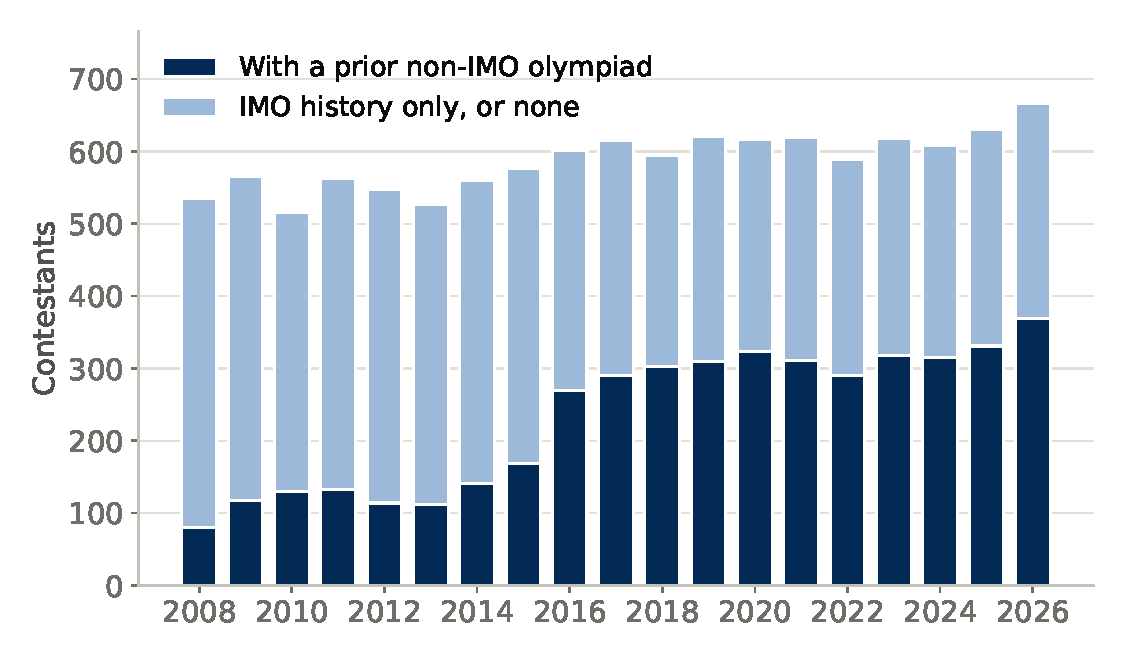
\includegraphics[width=\linewidth]{contestants_per_year.pdf}

      {\footnotesize IMO contestants per year, by prior international history.}
    \column{0.40\textwidth}
      \footnotesize
      \begin{itemize}\setlength{\itemsep}{7pt}
        \item \textbf{58.6\%} of IMO entries have an earlier international
              result; \textbf{39.6\%} an earlier olympiad other than the IMO
        \item That share grows from \textbf{15\%} (2008) to \textbf{55\%} (2026),
              as regional olympiads and their data appear
        \item Most common prior events: an earlier \textbf{IMO} (37.8\%),
              \textbf{APMO} (14.9\%), \textbf{BMO} (13.2\%)
        \item Awards are balanced except gold: none 24.5\%, HM 25.3\%,
              bronze 24.5\%, silver 17.1\%, gold 8.6\%
              $\rightarrow$ macro-averaged metrics
      \end{itemize}
  \end{columns}
\end{frame}

% ── SLIDE 6: Descriptives II ──────────────────────────────────────────────────
\begin{frame}{Descriptive Statistics: Does Earlier Performance Carry Over?}
  \begin{columns}[T]
    \column{0.49\textwidth}
      \centering
      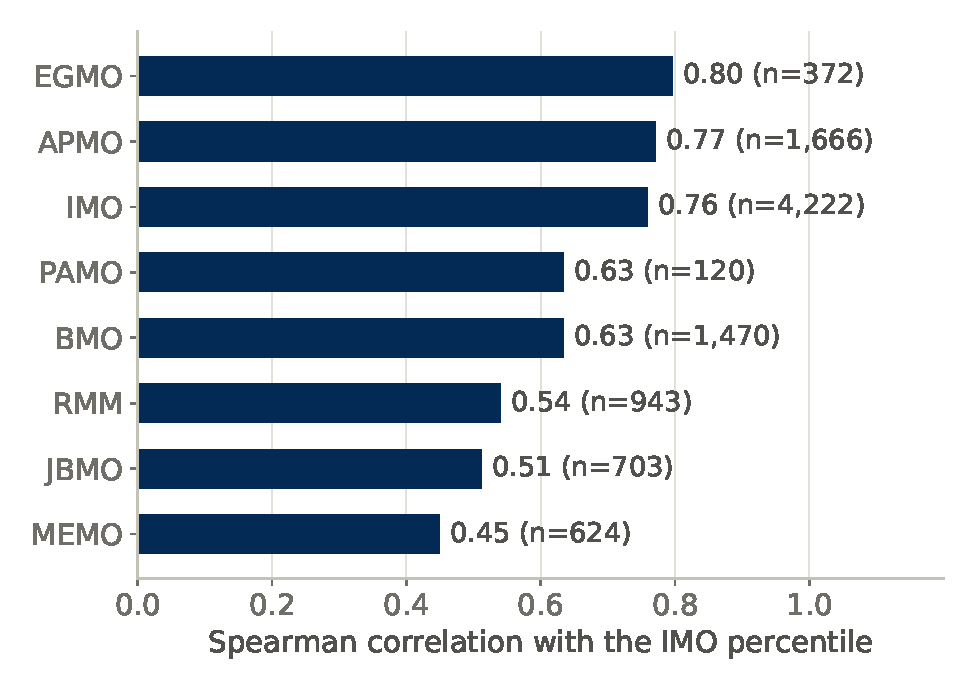
\includegraphics[height=0.52\textheight]{correlation_by_competition.pdf}

      \raggedright\footnotesize Best earlier percentile at each competition vs IMO percentile:
      \begin{itemize}\setlength{\itemsep}{1pt}
        \item \textbf{EGMO} (0.80), \textbf{APMO} (0.77) track the IMO as closely
              as an earlier IMO (0.76)
        \item Junior and regional contests less: JBMO 0.51, MEMO 0.45
      \end{itemize}
    \column{0.49\textwidth}
      \centering
      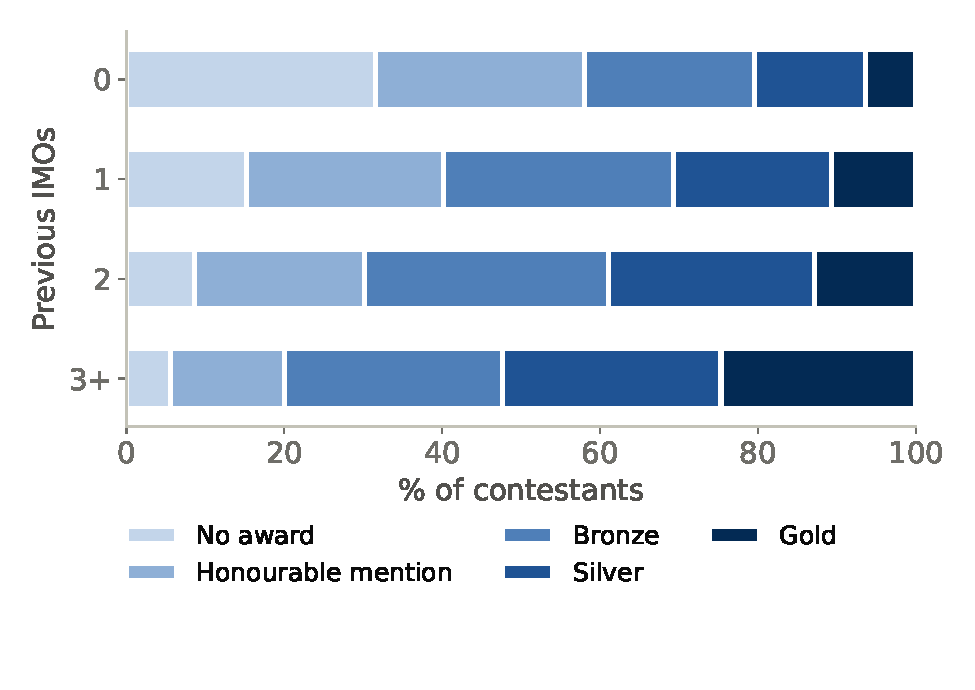
\includegraphics[height=0.52\textheight]{awards_by_prior_imo.pdf}

      \raggedright\footnotesize IMO award by number of earlier IMOs:
      \begin{itemize}\setlength{\itemsep}{1pt}
        \item Gold: \textbf{6\%} at a first IMO, \textbf{25\%} at a fourth or later
        \item Part of the signal is the country: strong countries dominate
              APMO and EGMO
      \end{itemize}
  \end{columns}
\end{frame}

% ── SLIDE 7: Data quality ─────────────────────────────────────────────────────
\begin{frame}{Data Quality: Validation and Coverage}
  \begin{columns}[T]
    \column{0.56\textwidth}
      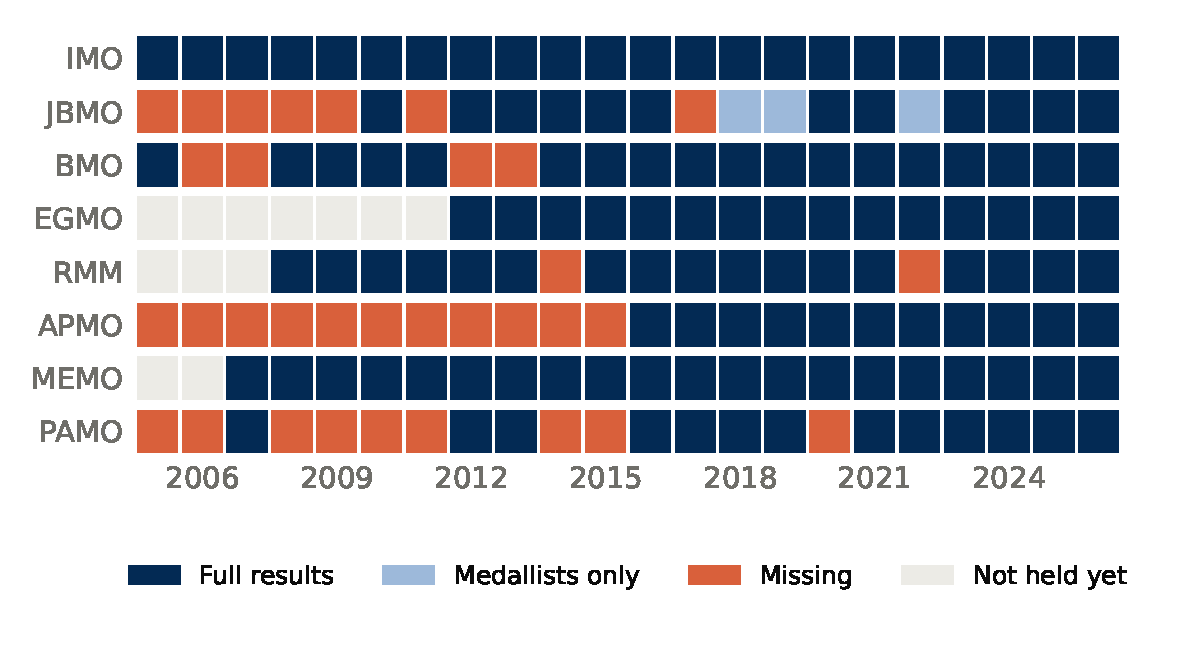
\includegraphics[width=0.94\linewidth]{coverage_matrix.pdf}

      \scriptsize
      \textbf{Known limitations:}
      \begin{itemize}\setlength{\itemsep}{1pt}
        \item Missing editions $\rightarrow$ \texttt{status = no\_data};
              APMO lists only the top 10 per country
        \item Month-level dates: same-year events use the usual month
        \item \textbf{Selection}: only IMO contestants are observed
      \end{itemize}
    \column{0.42\textwidth}
      \footnotesize
      \textbf{21 automatic checks}, each recomputed independently:
      \begin{itemize}\setlength{\itemsep}{2pt}
        \item one row per contestant and edition; scores in range
        \item \textbf{no future event} in any feature
        \item features and targets match a direct recomputation;
              every column documented
      \end{itemize}

      \vspace{6pt}
      \begin{block}{Errors found and fixed}
        \scriptsize
        \begin{itemize}\setlength{\itemsep}{2pt}
          \item \textbf{Identity}: 600 profiles of the same person merged,
                8 profiles mixing two people split
          \item \textbf{Country feature} used 1 year instead of 3
          \item \textbf{Trend feature} was extreme for events weeks apart;
                now computed per year
        \end{itemize}
      \end{block}
  \end{columns}
\end{frame}

% ── SLIDE 8: Baselines - setup ─────────────────────────────────────────────────
\begin{frame}{Baseline Models: Setup}
  \begin{columns}[T]
    \column{0.55\textwidth}
      \footnotesize
      \textbf{Two prediction tasks} for each contestant at an IMO:
      \begin{itemize}\setlength{\itemsep}{1pt}
        \item the \textbf{total score}, 0--42 (regression)
        \item the \textbf{award}: none, HM, bronze, silver, gold (classification)
      \end{itemize}

      \vspace{4pt}
      \textbf{Models}, from no information to all 20 compact features:

      \vspace{2pt}
      \scriptsize
      \setlength{\tabcolsep}{3pt}
      \begin{tabular}{L{2.6cm}L{5.0cm}}
        \toprule
        \textbf{What the model knows} & \textbf{Predicts for every contestant\,\dots} \\
        \midrule
        Nothing {\color{gray}(training mean / majority class)} & the average score (15.1) / the most
                                          frequent award (HM): the floor to beat \\[2pt]
        Only the country {\color{gray}(country history)} & their country's mean IMO score / most
                                          frequent award over the previous 3 IMOs \\[2pt]
        Country + own history {\color{gray}(linear / logistic regression)} & a weighted combination of earlier IMOs,
                                          other olympiads, team and country features \\
        \bottomrule
      \end{tabular}

    \column{0.43\textwidth}
      \begin{block}{Testing on the future}
        \footnotesize Train on IMO 2008--2022 (8,646 entries), test on
        \textbf{IMO 2023--2026} (2,523), never shuffled: the model predicts later
        IMOs from earlier ones, as it would in practice.
      \end{block}

      \vspace{6pt}
      \footnotesize
      \textbf{Metrics}
      \begin{itemize}\setlength{\itemsep}{2pt}
        \item Score: MAE (points), $R^2$
        \item Award: accuracy, accuracy within one award, \textbf{macro-F1}
              (gold is only 8\% of contestants)
        \item 95\% bootstrap intervals over test contestants
      \end{itemize}
  \end{columns}
\end{frame}

% ── SLIDE 9: Baselines - results ───────────────────────────────────────────────
\begin{frame}{Baseline Models: Results on IMO 2023--2026}
  \scriptsize
  \setlength{\tabcolsep}{5pt}
  \renewcommand{\arraystretch}{1.1}
  \textbf{\footnotesize Predicting the score (0--42)}

  \vspace{2pt}
  \begin{tabular}{L{3.6cm}L{4.4cm}cc}
    \toprule
    \textbf{What the model knows} & \textbf{What it predicts} & \textbf{MAE (points)} & \textbf{$R^2$} \\
    \midrule
    Nothing                         & 15 points for everyone                   & 8.4 & $\approx 0$ \\
    Only the country                & country's mean, last 3 IMOs             & 5.0 & 0.60 \\
    \textbf{Country + own history}  & regression on 20 features                & \textbf{4.4} & \textbf{0.70} \\
    \bottomrule
  \end{tabular}

  \vspace{8pt}
  \textbf{\footnotesize Predicting the award (none, HM, bronze, silver, gold)}

  \vspace{2pt}
  \begin{tabular}{L{3.6cm}L{4.0cm}ccc}
    \toprule
    \textbf{What the model knows} & \textbf{What it predicts} & \textbf{Accuracy} & \textbf{Within one award} & \textbf{Macro-F1} \\
    \midrule
    Nothing                         & HM for everyone                     & 25\% & 74\% & 0.08 \\
    Only the country                & country's usual award               & 47\% & 91\% & 0.46 \\
    \textbf{Country + own history}  & regression on 20 features           & \textbf{52\%} & \textbf{91\%} & \textbf{0.51} \\
    \bottomrule
  \end{tabular}

  \vspace{8pt}
  \footnotesize
  \begin{itemize}\setlength{\itemsep}{2pt}
    \item \textbf{The country explains most}; own history cuts the error from 5.0 to 4.4 points
    \item \textbf{Middle awards are hardest}: gold right 75\% of the time, silver only 33\%
    \item \textbf{History helps most where it exists}: compared with the country alone, the error
          drops by 0.67 points for contestants with earlier results, 0.49 for first-timers
  \end{itemize}
\end{frame}

% ── SLIDE 10: Intended analyses ───────────────────────────────────────────────
\begin{frame}{Intended Analyses (Phase 2)}
  \scriptsize
  \setlength{\tabcolsep}{4pt}
  \renewcommand{\arraystretch}{1.15}
  \begin{tabular}{L{3.3cm}L{5.4cm}L{4.6cm}}
    \toprule
    \textbf{Question} & \textbf{What we will do} & \textbf{What we learn} \\
    \midrule
    \textbf{RQ1}: How well can IMO results be predicted?
      & Tree models (random forest, gradient boosting) on all 97 features; they handle
        missing history and interactions. An ordinal model for the award (none $<$ HM
        $<$ \dots\ $<$ gold)
      & How far beyond the baselines (MAE 4.4, $R^2$ 0.70) individual history goes \\[4pt]
    \textbf{RQ2}: Which earlier competitions matter most?
      & SHAP values: each feature's contribution to each prediction, summed per
        competition. Then retrain without one competition at a time
      & A ranking of JBMO, BMO, EGMO, RMM, APMO, \dots\ by the information they add \\[4pt]
    \textbf{RQ3}: For whom do predictions fail?
      & Prediction errors by continent, access to regional olympiads, prior history,
        missing data, gender proxy; read the largest over- and under-predictions
      & Whether errors are systematic, e.g.\ larger for countries without
        regional olympiads \\
    \bottomrule
  \end{tabular}

  \vspace{2pt}
  \begin{columns}[T]
    \column{0.62\textwidth}
      \begin{block}{Also planned}
        \scriptsize
        \begin{itemize}\setlength{\itemsep}{1pt}
          \item Predict $z$-scores, which remove differences in difficulty between years
          \item Per-problem targets: is the hardest problem (P3 / P6) predictable?
          \item Report (max.\ 10 pages) and final presentation
        \end{itemize}
      \end{block}
    \column{0.36\textwidth}
      \vspace{14pt}
      \centering\scriptsize Code and data:\\
      \texttt{github.com/AnaBogdan05/\\imo-results-predictor}
  \end{columns}
\end{frame}

% ── Thanks ───────────────────────────────────────────────────────────────────
{
\setbeamertemplate{headline}{}
\begin{frame}
  \begin{center}
    \vspace{1.5cm}
    {\color{nlpblue}\Large\bfseries Thank you for your attention!}

    \vspace{1.2cm}
    {\color{nlpblue!30}\rule{0.5\textwidth}{0.4pt}}
    \vspace{1.2cm}

    {\normalsize\textbf{Ana-Maria-Iulia Bogdan}}\\[8pt]
    {\footnotesize\color{nlpblue} ana\_maria.bogdan@stud.acs.upb.ro}
  \end{center}
\end{frame}
}

\end{document}
